\documentclass[12pt,a4paper,oneside]{article}
\usepackage[colorlinks=true,unicode]{hyperref}
\usepackage[utf8]{inputenc}
\usepackage[czech]{babel}
\usepackage{graphicx}
\usepackage{pdfpages}
\textwidth 16cm \textheight 25cm
\topmargin -1.3cm 
\oddsidemargin 0cm
\usepackage{footnote}
\pagestyle{empty}
\begin{document}
\title{Dělička hodin s differenčním vstupem }
\author{Jakub Kákona, Martin Kákona, kaklik@mlab.cz}
\maketitle

\thispagestyle{empty}
\begin{abstract}
Může být nastaveno více dělících poměrů. Možnosti jsou ($\div$1, $\div$2, $\div$4, $\div$8) nebo ($\div$2, $\div$4, $\div$8, $\div$16). EN vstup je synchronní s interními hodinami, proto dojde k vypnutí výstupu při návratu na nulu.
\end{abstract}

\begin{figure} [htbp]
\begin{center}
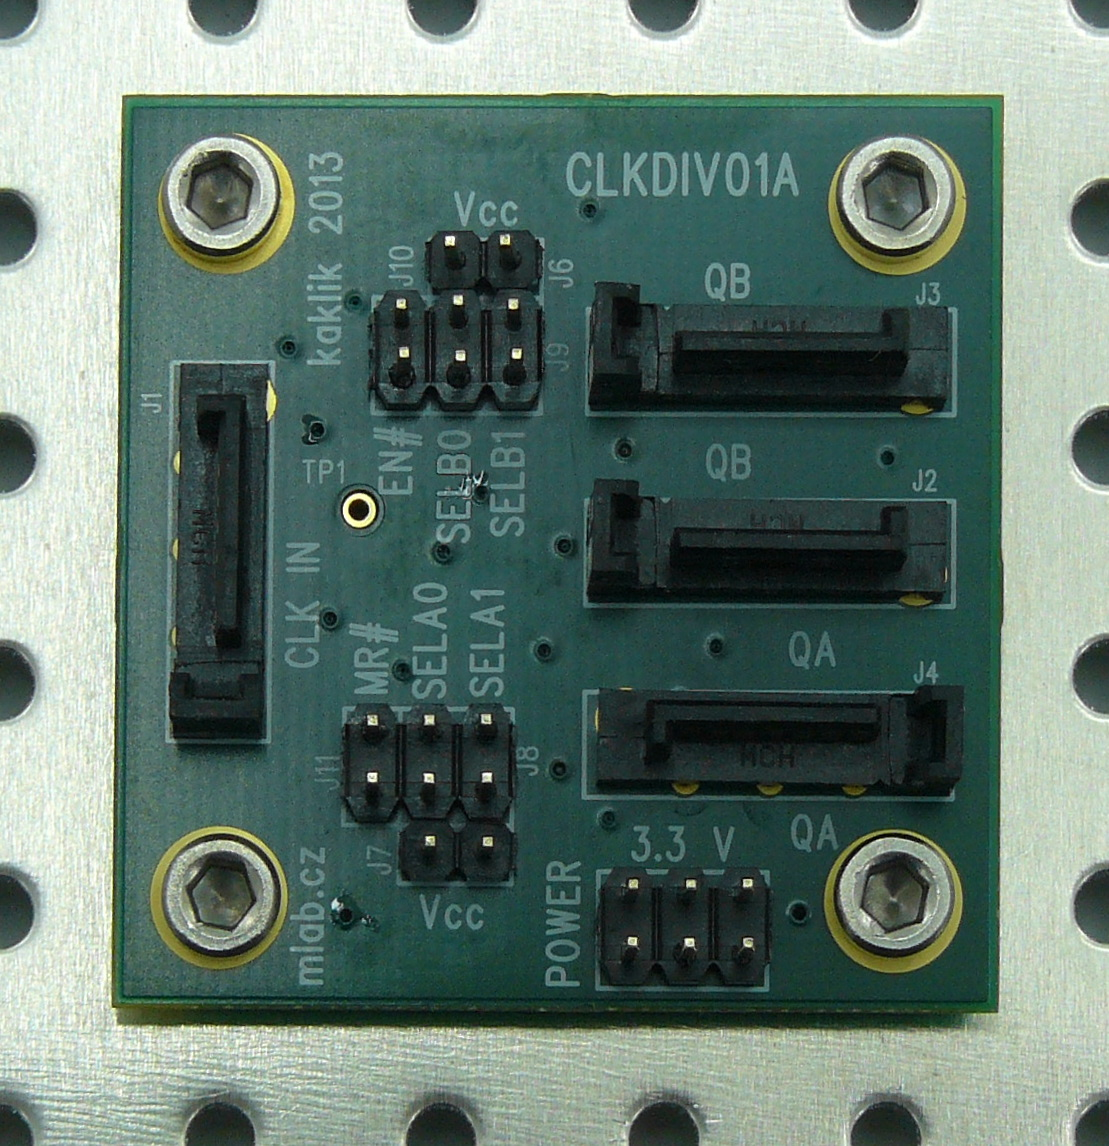
\includegraphics [width=80mm] {./img/CLKDIV01A_Top_Big.jpg} 
\end{center}
\end{figure}

\begin{figure} [b]

\includegraphics [width=25mm] {./img/CLKDIV01A_QRcode.png} 
\end{figure}

\newpage
\tableofcontents


\section{Technické parametry}
\begin{table}[htbp]
\begin{center}
\begin{tabular}{|c|c|c|}
\hline
\multicolumn{1}{|c|}{Parametr} & \multicolumn{1}{|c|}{Hodnota} & \multicolumn{1}{|c|}{Poznámka} \\ \hline
Napájecí napětí & 3.3 V &  cca 100 mA \\ \hline
Typy vstupní diff logiky  & LVDS, LVPECL, CML, HSTL, HCSL & \\ \hline
Logika řídících signálů  & LVTTL, LVCMOS & \\ \hline
Pracovní frekvence vstupu  & $<$ 3 GHz & \\ \hline
Dělící poměry QA & $\div$1, $\div$2, $\div$4, $\div$8 & \\ \hline
Dělící poměry QB & $\div$2, $\div$4, $\div$8, $\div$16 & \\ \hline
\end{tabular}
\end{center}
\end{table}

\newpage
\section{Popis konstrukce}

\subsection{Zapojení}

Zapojení modulů je identické s doporučeným zapojením z katalogového listu. Vstupy a výstupy jsou vyvedeny na differenční signály SATA konektorů. Řídící signály lze ovládat přímo z procesoru připojením výstupního pinu na hřebínek, nebo lze dělící poměr navolit pevně Jumpery. 

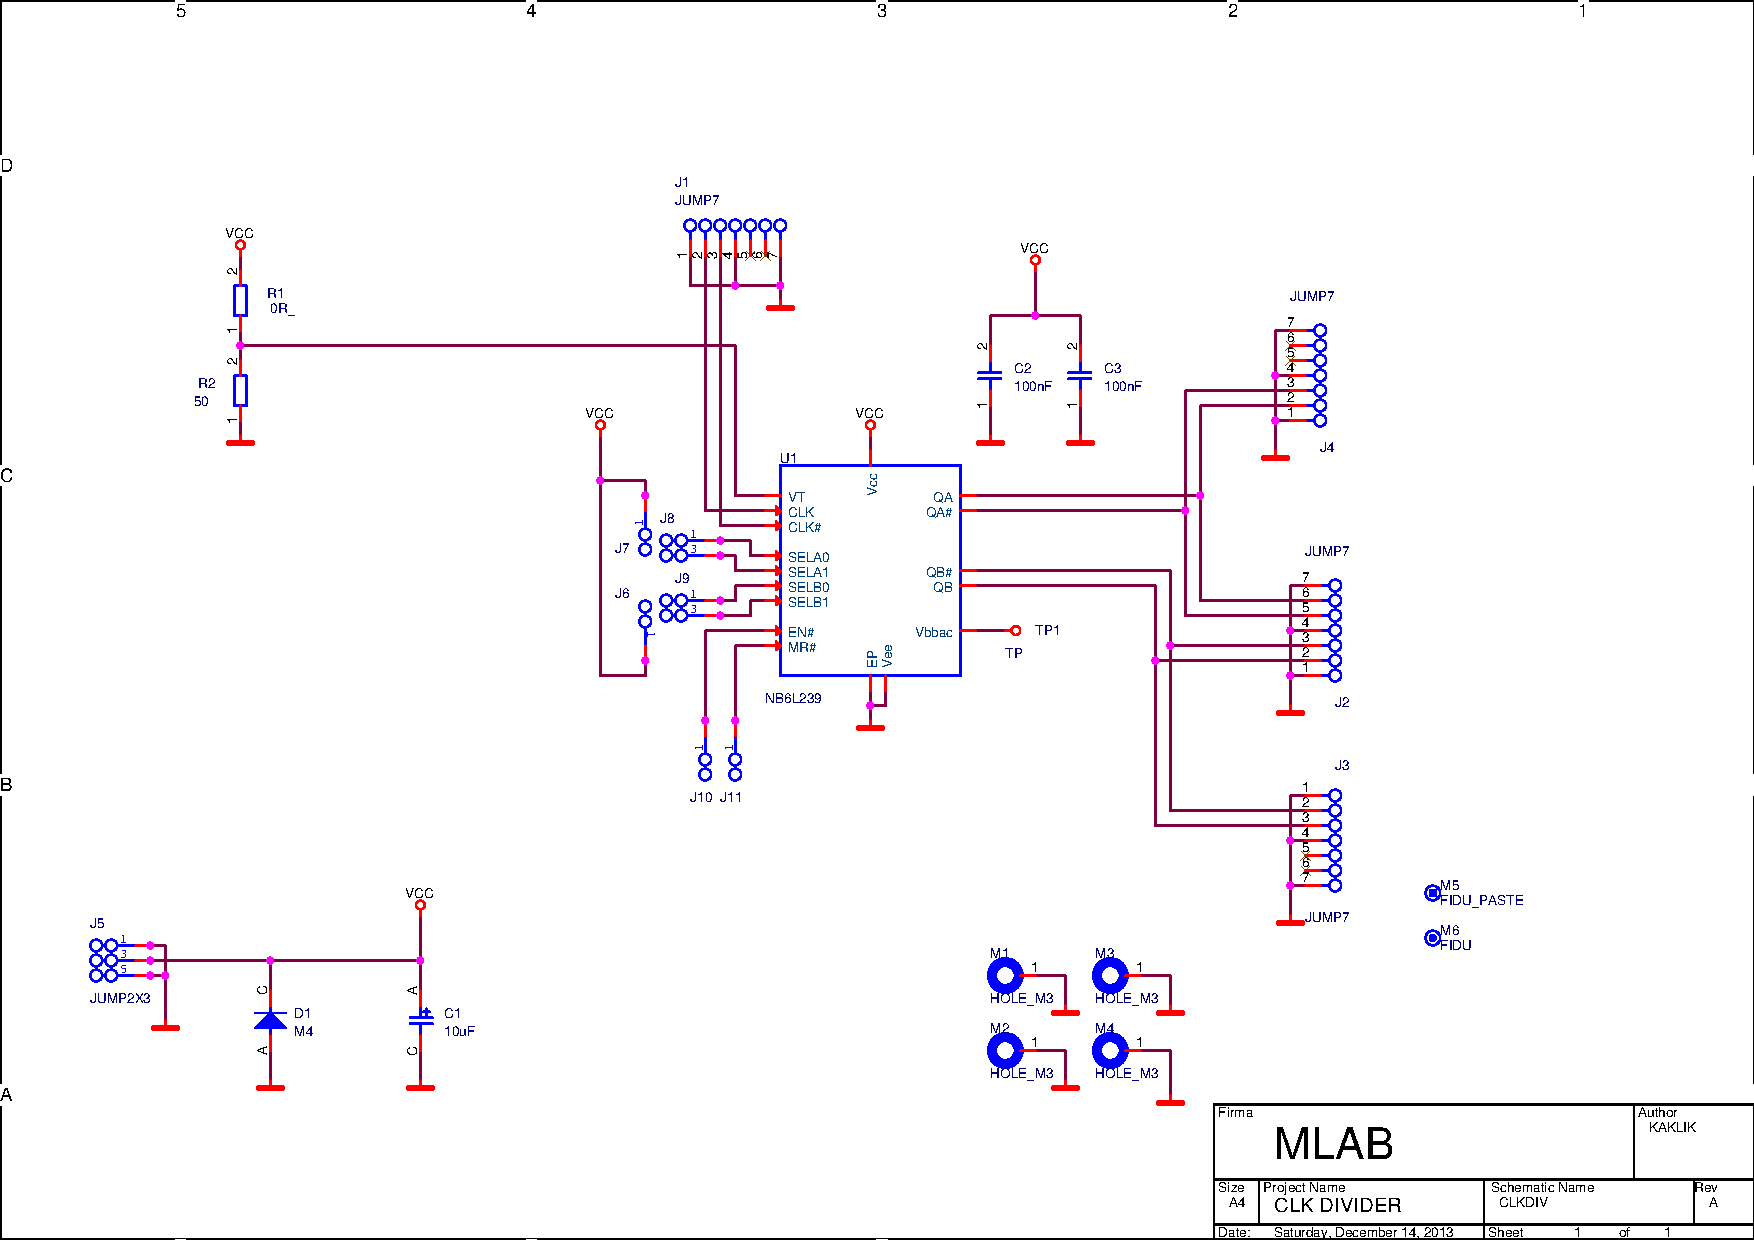
\includepdf[pages={1},landscape=true]{../../SCH/clkdiv.pdf}

\subsection{Odrušení}

Tento modul může produkovat rušení v napájení. Je proto vhodné jej v citlivých analogových aplikacích připojovat krátkým napájecím kablíkem.

\section{Výroba a testování}

\subsection{Osazení}

%\begin{figure} [h!tbp]
%  \centering
%  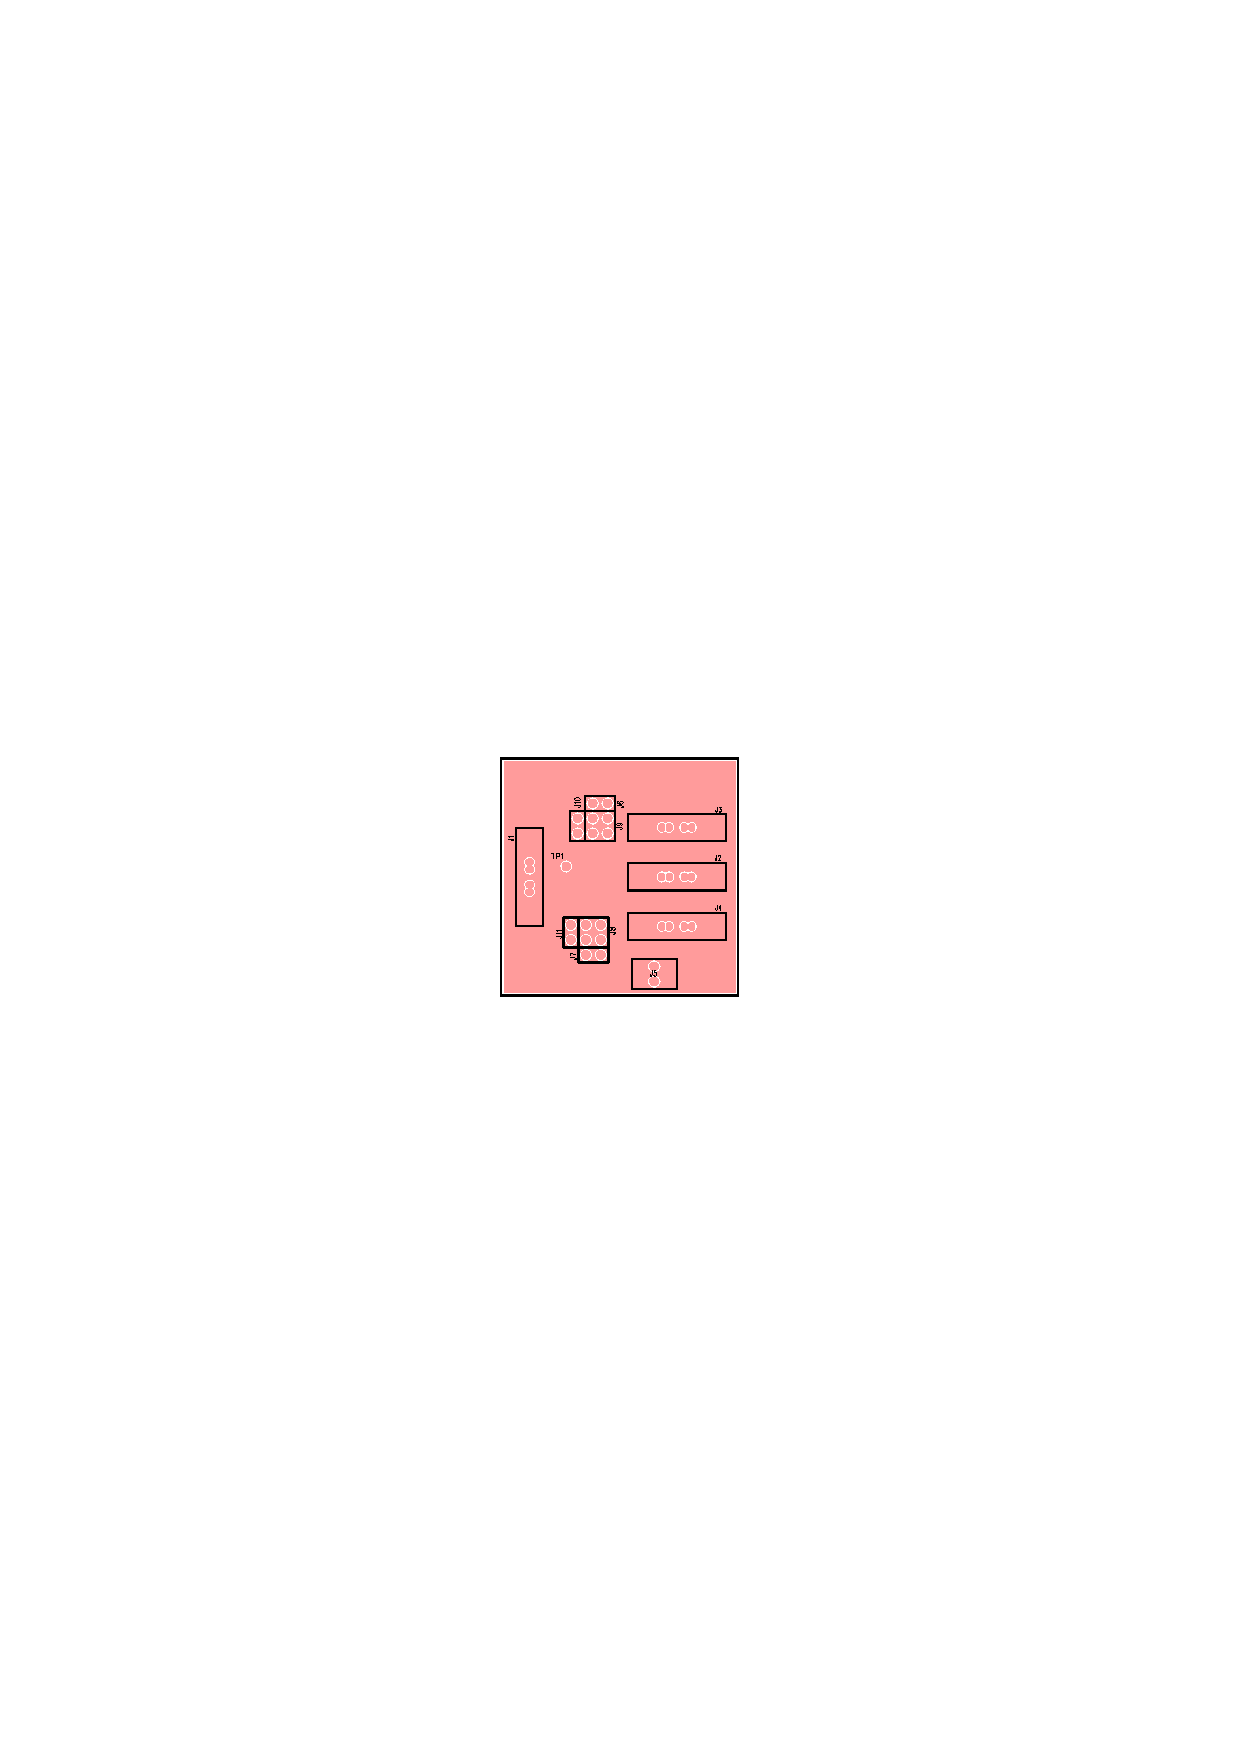
\includegraphics[trim = 6.5cm 11.5cm 6.5cm 11.5cm, clip, width=10cm]{../../CAM_DOC/O1.pdf}
%  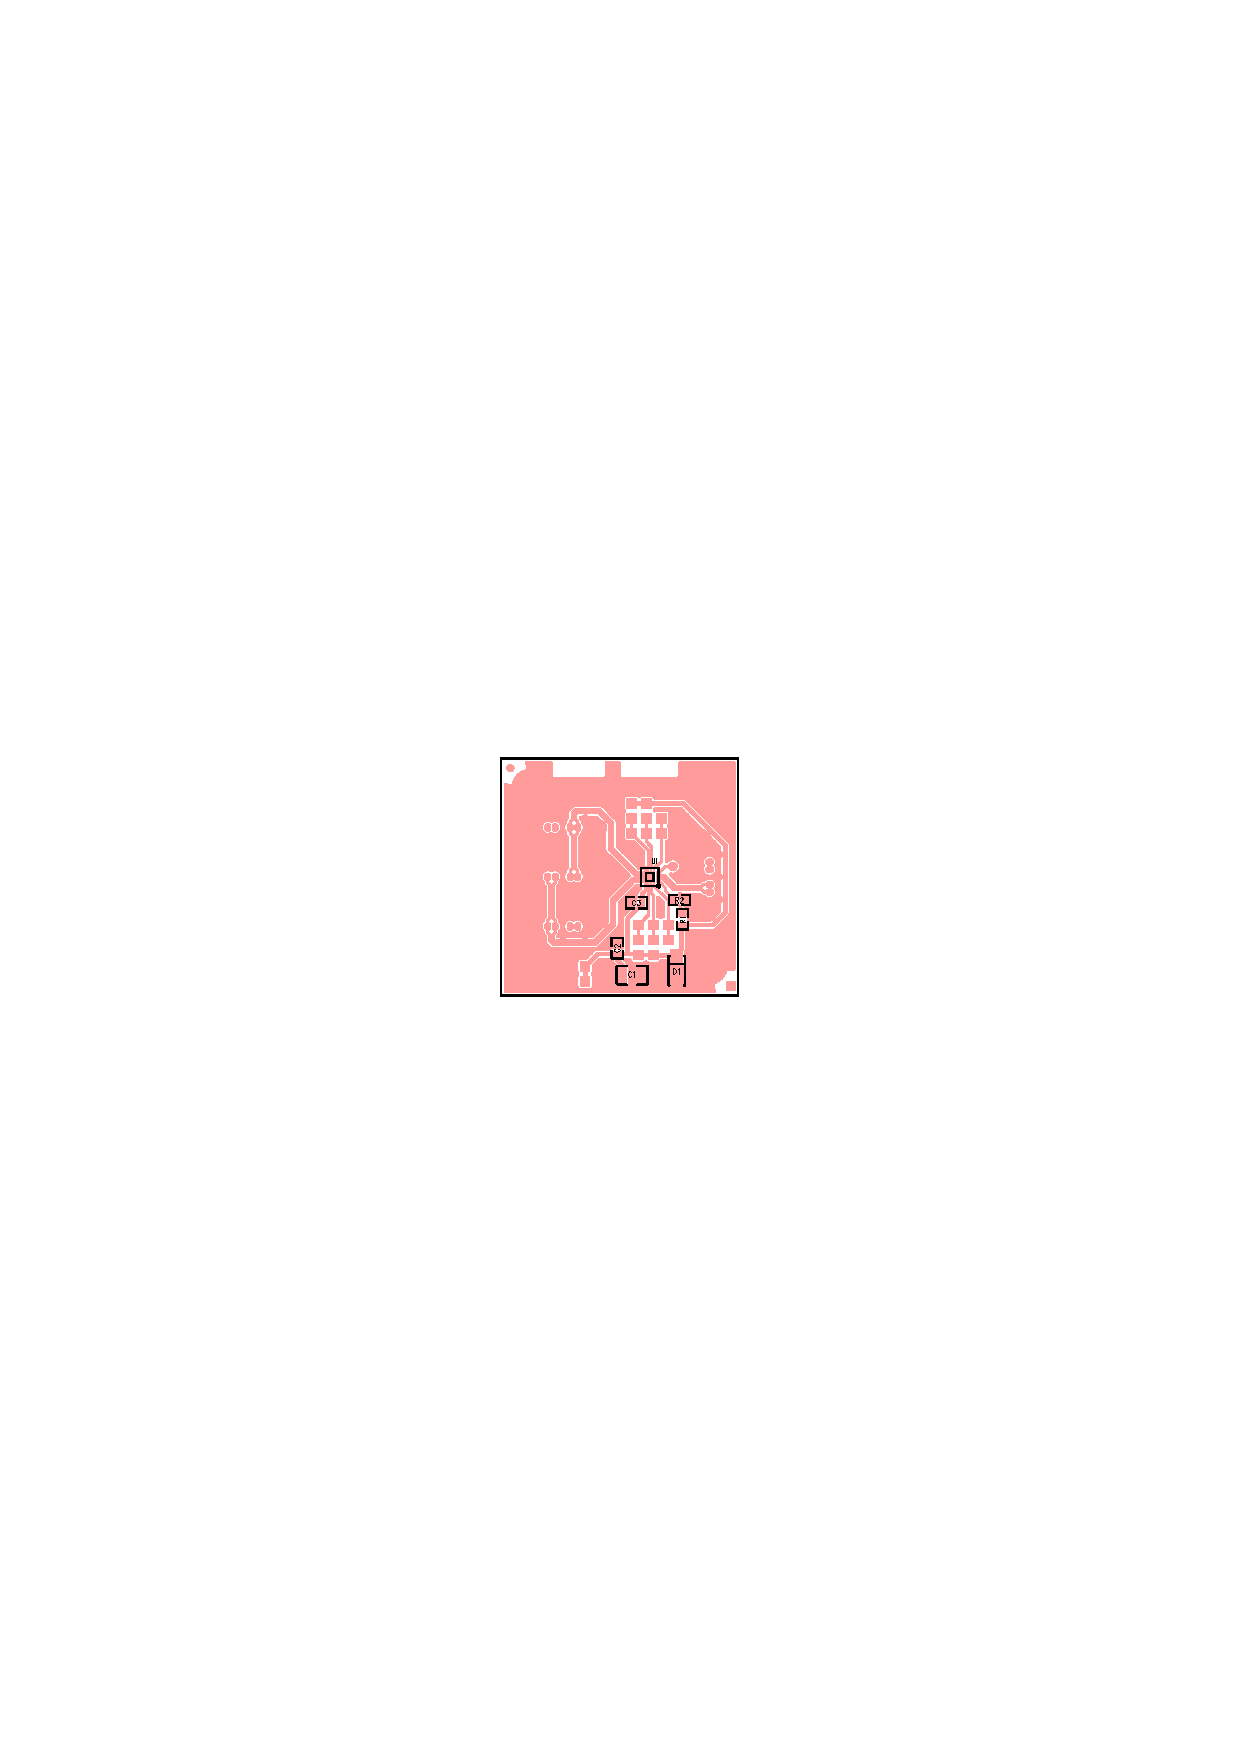
\includegraphics[trim = 6.5cm 11.5cm 6.5cm 11.5cm, clip, width=10cm]{../../CAM_DOC/O2.pdf}
%  \caption{Osazovací plán horní a spodní strany plošného spoje}
%  \label{fig:osazovaci_plan}
%\end{figure}

\section{Programové vybavení}

\begin{thebibliography}{99}
%\bibitem{DR2G}{Původní konstrukce} 
%\href{http:// odkaz na nejakou zajimavou konstrukci}{odkaz na nejakou zajimavou konstrukci}

\end{thebibliography}
\end{document}